% !TeX spellcheck = de_DE
\documentclass[11pt]{scrartcl}
\usepackage[utf8]{inputenc}
\usepackage[german]{babel}
\usepackage[T1]{fontenc}
\usepackage{latexsym}
\usepackage{stmaryrd}
\usepackage{amsmath}
\usepackage{amssymb}
\usepackage{amsxtra}
\usepackage[square,authoryear]{natbib}
\usepackage{listings}
\usepackage{url}
\usepackage{hyperref}
\usepackage{graphicx}
\usepackage{color}
\usepackage{listings}
\usepackage{textcomp}

\definecolor{listinggray}{gray}{0.5}
\definecolor{lbcolor}{rgb}{0.9,0.9,0.9}
\lstset{
	backgroundcolor=\color{lbcolor},
	tabsize=4,
	rulecolor=,
	language=Cobol,
	basicstyle=\scriptsize,
	upquote=true,
	aboveskip={1.5\baselineskip},
	columns=fixed,
	showstringspaces=false,
	extendedchars=true,
	breaklines=true,
	frame=single,
	showtabs=false,
	showspaces=false,
	showstringspaces=false,
	identifierstyle=\ttfamily,
	keywordstyle=\color[rgb]{0,0,1},
	commentstyle=\color[rgb]{0.133,0.545,0.133},
	stringstyle=\color[rgb]{0.627,0.126,0.941},
}

\newcommand{\ncite}{\footnote{Citation needed}}
\newcommand{\lb}{\\ \\}

\newtheorem{theorem}{Theorem} 
\newtheorem{definition}[theorem]{Definition} 

\renewcommand*{\lstlistlistingname}{Quellcodeverzeichnis}
\renewcommand*\lstlistingname{Quellcode-Beispiel}

\setlength{\parindent}{0em}

\begin{document}
	
% === TITLE PAGE ===
\title{Ans"atze und Verfahren der Datenmigration}

\subtitle{Datenmigration im Kontext des Reengineering} 

%\author{Julian Schenkemeyer, Tobias Fechner\\
%	{\texttt{\{5Schenke,1fechner\}@informatik.uni-hamburg.de}}}

\date{Modul Software Reengineering 2015/2016\\
  \small Fachbereich Informatik\\ 
  Arbeitsbereich Softwarekonstruktion \& Werkzeuge\\ 
  Universit"at Hamburg\\[4mm]
  \today}

\maketitle

% === ABSTRACT ===
\begin{abstract}
	\small\noindent\textbf{Abstract}

	\noindent Die Erhaltung von Daten aus dem Kontext von Legacy-Systemen spielt eine entscheidende Rolle beim Reengineering von Software. Auswahl, Extraktion und Konvertierung vorhandener Daten in ein neues Umfeld sind nur einige der T"atigkeiten der Datenmigration. \\
	Unterschiedliche Strategien zur Migration von Daten setzen unterschiedliche Schwerpunkte um diese ihrem Kontext entsprechend durchf"uhren zu k"onnen. Die Betrachtung aus Sicht sowohl der Datenquellen als auch der umliegenden Anwendungssysteme bildet den Kern dieser Strategien. Unterschiedliche Strategien kommen dabei in verschiedenen Situationen zum Einsatz und besitzen jeweils eigene Vor- und Nachteile. \\
	Dar"uber hinaus bildet die Datenmigration ein hohes Risiko für das Unternehmen. Um dieses Risiko zu reduzieren, existieren verschiedene Prozessmodelle. Diese versuchen, den Ablauf der Datenmigration in einzelne Phasen zu strukturieren und die jeweiligen Kernaufgaben zu identifizieren. Sie bilden die Grundlage für die Entscheidung, welche der unterschiedlichen Vorgehensweisen für die Datenmigration an effektivsten und mit dem geringsten Risiko durchzuf"uhren ist. \\
	Die Vorgehensweisen beleuchten dabei die technische Prozedur der Datenmigration vom Legacy-System zum neuen System. Zu entscheiden ist, ob eine schrittweise oder komplette Migration durchgef"uhrt werden soll. Beide Ans"atze eignen sich nicht f"ur jedes System. Sie m"ussen f"ur eine erfolgreiche Datenmigration mit Bedacht gewählt werden.\\
	Ziel dieser Ausarbeitung ist es, die allgemeine Thematik der Datenmigration zu erl"autern, sowie Strategien, Prozessmodelle und Vorgehensweisen vorzustellen.
\end{abstract}

\newpage

\tableofcontents

\newpage

\listoffigures
\listoftables
\lstlistoflistings
\newpage

% ===========================================================================================================
% ======= BEGIN CONTENT =====================================================================================
% ===========================================================================================================

% !TeX spellcheck = de_DE
\section{Einleitung}
\label{chapter:einleitung}

%\huge
%\textbf{Aufgabenstellung: Bewerten Sie Ansätze der Datenmigration bezüglich Stärken, Schwächen, Einsatzbereich!} 
%\normalsize
%\lb

Die Datenmigration spielt im Kontext des Software-Reengineering eine entscheidende Rolle. Basis vieler Softwaresysteme bilden dynamische Daten in unterschiedlichen Formaten und auf Basis unterschiedlicher Technologien. Gesch"aftsprozesse basieren h"aufig auf bestimmten Datenstrukturen und -schemata. Als Migration bezeichnet man dabei das Verlagern von Daten auf andere Medien, das Konvertieren in neue Formate und die Restrukturierung bereits vorhandener Daten \citep{morris-2012}. Die Anpassung der umliegenden Software-Systeme spielt dabei eine wichtige Rolle \citep{henrard-2002}.
\lb
Konkret werden im Kontext der Datenmigration vorhandene Daten f"ur das Reengineering von Software verwertet. Wichtige Kunden- oder Gesch"aftsdaten m"ussen auch nach Reengineering, Anpassung und Neuentwicklung von Softwaresystemen weiterhin genutzt werden k"onnen. Ein strukturiertes Vorgehen bei der Analyse, Konvertierung, Portierung und Anpassung dieser Daten bildet die Grundlage der Datenmigration.  
\lb
Unterschiedliche Strategien versuchen auf verschiedenen Ebenen, die Migration von Daten zu strukturieren. Im Kontext des Reengineering von Daten m"ussen nicht alleine Datenquellen und -schemata angepasst werden. Im Zusammenhang mit urspr"unglichen Daten entwickelte Legacy-Systeme m"ussen neuen Datenquellen angepasst und entsprechend adaptiert werden \citep{henrard-2002}.	
\lb
F"ur Durchf"uhrung und Einf"uhrung der Datenmigration im Kontext von Legacy-Systemen existieren verschiedene Ans"atze. Diese versuchen den Ablauf von Migrationsprojekten mittels Prozessmodellen zu strukturieren. Ein allgemeines Prozessmodell, das auf jedes Unternehmen ohne entsprechende Anpassungen angewandt werden kann, existiert jedoch nicht. Nur wenn alle Gegebenheiten und Abl"aufe des Unternehmen betrachtet werden, kann eine erfolgreiche Migration mit minimalen Risiko durchgef"uhrt werden \citep{wuLawless-1997} \citep{ackermann-2005}.
\lb
Aus einer Vielfalt von Ans"atzen und Strategien ergeben sich je entsprechende Vor- und Nachteile. Schon eine grobe Analyse zeigt St"arken und Schw"achen der jeweiligen Methodiken. Unterschiedliche Ebenen f"ur die Anwendung der Strategien lassen sich auf verschiedene Anwendungsbereiche und Beteiligte zur"uckf"uhren.
\lb
Der Rest dieser Ausarbeitung ist wie folgt strukturiert: Kapitel \ref{chapter:motivation} beschreibt die Datenmigration im Kontext des Reengineering und gibt Hinweise auf die Wichtigkeit und Relevanz der Durchf"uhrung. Kapitel \ref{chapter:richtlinien} stellt einen generellen unangepassten Ablauf einer Migration mit seinen jeweiligen T"atigkeiten vor. Kapitel \ref{chapter:strategien} stellt Strategien der Datenmigration auf zwei Ebenen vor und beschreibt deren Vor- und Nachteile sowie deren Einsatzbereich und Kapitel \ref{chapter:vorgehensweisen} beschreibt das Vorgehen bei der Einf"uhrung der Ergebnisse der Datenmigration. Abschlie"send gibt Kapitel \ref{chapter:fazit} eine b"undige Zusammenfassung der Inhalte.
% !TeX spellcheck = de_DE
\section{Motivation}
%TODO Tobias
%http://www.dtic.upf.edu/~jbisbal/publications/icsc97.pdf
%http://www.aifb.kit.edu/images/2/27/2002_14_Stojanovic_A_reverse_engin_1.pdf 	%Kann eventuell verwendet werden, als inspiration f"ur Szenario?
%http://edepositireland.ie/bitstream/handle/2262/27040/The%20Butterfly%20Methodology%20a%20gateway-free%20approach%20for%20migrating%20legacy%20information%20systems.pdf?sequence=1&isAllowed=
%http://www.dtic.upf.edu/~jbisbal/publications/datasem97.pdf
%http://csis.pace.edu/~marchese/CS775/Proj1/legacyinfosys_directions.pdf
%http://www.tara.tcd.ie/bitstream/handle/2262/27050/An?sequence=1
%http://www.oracle.com/technetwork/middleware/oedq/successful-data-migration-wp-1555708.pdf
%http://searchsmbstorage.techtarget.com/tip/Data-migration-strategies-and-best-practices
%https://pure.fundp.ac.be/ws/files/168599/wcre02.pdf
%http://www.dtic.upf.edu/~jbisbal/publications/datasem97.pdf
%http://csis.pace.edu/~marchese/CS775/Proj1/legacyinfosys_directions.pdf
%http://www.tara.tcd.ie/bitstream/handle/2262/27050/An?sequence=1
%http://ieeexplore.ieee.org/stamp/stamp.jsp?tp=&arnumber=271615 ==> IEEE Xplore Data Migration von Cheong Youn, Cyril S. Ku
%http://www.oracle.com/technetwork/middleware/oedq/successful-data-migration-wp-1555708.pdf

%\begin{itemize}
%	\item Warum ist Datenmigration besonders wichtig bei Reengineering?
%	\item General Scenario
%	\item Ans"atze grob einf"uhren
%	\item Migration als Erhaltung von Daten
%	\item Etwa wichtige Kunden- oder Transaktionsdaten von Banken
%	\item Daten werden weiterhin verwendet, System m"ussen (technisch oder fachlich) erneuert werden
%	\item Die bereits vorhandenen Daten werden u.U. anders genutzt oder erfordern Anpassungen
%	\item Risiken der Datenmigration
%\end{itemize}
%\subsection{Reengineering}

Als zentrale Rolle des Reengineering von Software versteht sich eine ''Untersuchung (Reverse Engineering) und Änderung des Systems, um es in neuer Form zu implementieren'' \citep{chikofsky-1990}. In diesem Zusammenhang versucht das Konzept der Datenmigration eben dieses Ziel im Hinblick auf bereits vorhandene Daten zu erreichen. Gesch"aftskritische Daten bilden einen wichtigen Bestandteil vieler Softwaresysteme. Legacy-Systeme bauen h"aufig auf primitiven Mitteln zur Datenhaltung auf \citep{henrard-2002}.
\lb 
Unterschiedliche Ans"atze der Datenmigration finden in spezifischen Kontexten Anwendung. Je nach Anwendungsgebiet der Migration existieren Techniken und Vorgehensweisen f"ur die Datenmigration. Diese unterscheiden sich in den einzusetzenden Hilfsmitteln, Beteiligen sowie Auswirkungen auf andere Systemteile. Direkte Auswirkungen zeigen sich dabei in umliegenden Softwaresystemen, welche auf die Nutzung der Daten angewiesen sind.
\lb
Die Planung von Datenmigration stellt meist nur einen Teil des Reengineerings von Softwaresystemen dar. Innerhalb entsprechender Projekt folgt sinnvollerweise auch der Subprozess der Datenmigration entsprechenden Schemata. %TODO Ergaenzen um Projekt-geschwafel
\lb
Einf"uhrungsstrategien bildet konzeptionell den Abschluss der Datenmigration. Nach erfolgen Analysen, Tests und entsprechenden Anpassungen in den betroffenen Systemen kann die Einf"uhrung der "Anderungen mehreren Mustern folgen. 

\subsection{Datenmigration}

%TODO Definition erl"autern??
\begin{quote}''Data migration is the selection, perparation, extraction, transformation and permanent movement of appropriate data that is of the right quality to the right place at the right time and the decommissioning of legacy data stores'' \flushright\citep[S.~7]{morris-2012}
\end{quote}

Eine Strukturierung von Daten au"serhalb von Softwaresystemen bildet h"aufig den Kern wichtiger Gesch"aftsprozesse. Auf der zugrundeliegenden Dynamik externer Datenquellen skalieren die Aufgaben unterschiedlichster Softwaresysteme. Durch das Vorhalten von Daten in externen Quellen k"onnen Informationen zur Laufzeit der System dynamisch nachgeladen und persistiert werden.
\lb
Das Reengineering von Software beinhaltet meist nicht alleine eine Restrukturierung von Softwaresystemen. Zugrundeliegende Daten sind auf die Nutzung und den speziellen Kontext des Systems ausgelegt. Hohe Anforderungen an Stabilit"at und Verl"asslichkeit machen diese Daten zu einer zentralen Komponente von Legacy-Systemen.
\lb
Anders als eine Portierung von Software oder Systemen beruft sich die Datenmigration somit auf das verschieben und Restrukturieren von Daten.
\lb
Aus ihrer zentralen Rolle innerhalb von Legacy-Systemen leitet sich ein hoher Gesch"aftswert der Daten ab. Beispiele finden sich etwa in Form von Daten der Kunden einer Bank, dem Katalog von Warenh"ausern oder einer Verwaltung von St"uckg"utern im Betrieb von Containerterminals. 
\lb
Datenmigration erfasst vorrangig Daten im Allgemeinen Sinne. Dies reicht von Datenbanken, Gesch"aftsdaten in Excel-Tabellen bis hin zu eigenen Datenformaten. Ziel der Migration ist vorrangig das Erhalten von Daten. Der Gesch"aftswert dieser Daten steht als zentrales Argument f"ur die Modernisierung von Datenhaltung und -management. Neben der physischen Migration von Daten, der Aktualisierung von Systemsoftware und letztendlich der Modernisierung der Modellierung der Daten reichen zahlreiche Ans"atze der Datenmigration. Die Integration der Migration erfordert eine Verzahnung mit Prozesses des Reengineering und der konstanten Nutzung von Legacy-Systemen.

\subsection{Szenario}
%TODO Das ist ja furchtbar, vielleicht f"allt dir da was besseres ein?

Um die Kernaufgaben und den Kontext der Datenmigration zu erl"autern, l"asst sich ein exemplarischer Anwendungsfall f"ur die Datenmigration im Kontext von Legacy-Systemen anf"uhren.
\lb
Kontext:
Ein Versicherungsunternehmen; Ein in COBOL verfasstes Legacy-System sowie ein System zum Datenmanagement auf Basis ISAM\footnote{\textit{Indexed Sequential Access Method}}. Die Aufgabe des Systems ist das Erfassen und Verwalten von Versicherungen. Kunden- und Vertragsdaten sind Grundlage f"ur die Arbeit des Systems. Die Datenmodellierung orientiert sich an den Gesch"aftsprozessen. 
\lb
Im Zug einer Evolution des Unternehmens soll das Softwaresystem neu entwickelt werden. Um bestehende Gesch"aftsprozesse korrekt abzubilden, erfolgt eine umfassende Analyse. Auf Basis dieser Daten soll das neue System implementiert werden. Da sich das neu Anwendungssystem "ahnlich zum bestehenden System verhalten soll, m"ussen bereits vorhandene Kunden- und Versicherungsdaten "ubertragen werden. Zu diesem Zweck muss die vorhandene Datenhaltung an das neue System angepasst werden. Neue technische und konzeptionelle "Uberlegungen erfordern unter Umst"anden neue Denkweisen bei der Nutzung von vorhandenen Kundendaten. Die Datenmigration schlie"st in diesem Kontext die Konvertierung und den "Ubertrag vorhandener Daten in das neue System ein.

\subsection{H"aufige Probleme}

Um die Relevanz von Datenmigration weiter hervorzuheben, erl"autert \citep{morris-2012} h"aufig Problem, die im Zuge der Datenmigration h"aufig auftreten. Im Jahr 2011 lagen etwa 40\% der Projekte zur Datenmigration au"serhalb von Zeit und Kostenplan, oder schlugen gesamtheitlich fehl \citep{howard-2011}.

\begin{itemize}
	\item \textbf{Technologiezentrierung} \\
			Datenmigration wird h"aufig untersch"atzt. Oft wird sie lediglich als Migration als technisches Problem verstanden \citep[S.~9]{morris-2012}
	\item \textbf{Mangel an Spezialisten} \\
			Die Analyse von Daten und die folgende Migration erfordert unter Umst"anden Spezialisten oder Analysten f"ur eine diffundierte Analyse. Eine Synthese aus fachlichen und technischen Problematiken kann im Kontext der Datenmigration eine saubere Trennung zwischen gesch"aftlichen und technischen Problemen erschweren.
	\item \textbf{Untersch"atzen der Datenmigration} \\
			Im Kontext von Legacy-Systemen ist die tats"achliche Tief vorhandener Daten potentiell unbekannt. Das Erfassen der dazu notwendigen T"atigkeiten kann so leicht untersch"atzt werden.
	\item \textbf{Problemzuweisung} \\
			Die Beziehungen zwischen (Migrations-)Projekt und allt"aglichem Gesch"afts sind selten eindeutig. Unkontrollierte Zuweisungen der Problem zu jeweils einem der Beteiligen kann unbeabsichtigt zur Rekursion bei der Zuweisung einzelner Problembereiche \citep[S.~9]{morris-2012}.
\end{itemize}

Hinweise f"ur die erfolgreiche Durchf"uhrung von Projekten zur Datenmigration finden sich etwa in \citep{sas-2009}, \citep{oracle-2011}. %TODO Etwas mehr...

% !TeX spellcheck = de_DE
\section{Strategien zur Datenmigration}
\label{chapter:strategien}
%TODO Tobias

Als Kernelement der Datenmigration stehen unterschiedliche Strategien zur Verf"ugung. Diese Ans"atze fokussieren dabei je die Ebenen Datenquellen und Anwendung\citep{henrard-2002}. Datenbanken und -quellen bilden die grundlegende Ebene. Schemata der Datenhaltung m"ussen angepasst und konvertiert werden. 
\lb
Auf Ebene der Anwendung m"ussen in Folge der Migration der Daten umliegende Softwaresysteme mit Zugriff auf diese Daten ihre Nutzung der Datenquellen anpassen. Da unter Umst"anden Schnittstellen und Datenformate ver"andert werden, muss die spezifische Nutzung dieser der Evolution auf Datenbankebene angepasst werden.
\lb
Einzelne Strategien bieten Vor- und Nachteile. Sie sind von unterschiedlichen Gruppen innerhalb eines Unternehmens oder Migrationsprojektes vorzunehmen.


% == 
\subsection{Datenbankebene}

Auf Ebene der Daten erfolgt sinnvollerweise eine Anpassung von zugrundeliegenden Technologien, Datenbankschemata oder Datenformaten. Gr"unde f"ur eine Migration auf dieser Ebene finden sich auf Ebene der Hintergr"unde des zugrundeliegenden Reengineerings. Sie reichen von einem Wechsel auf zukunftssichere Technologien oder einer Anpassung von Gesch"aftsprozessen. Unterschiedliche Ans"atze beg"unstigen oder hemmen dabei das Erreichen eben dieser Ziele. 

% ===
\subsubsection{Physisch}

Die Migration von Daten auf physischer Ebene schlie"st die Konvertierung von Datenformaten und -schemata auf rein struktureller Ebene ein. Daten werden dabei ohne Betrachtung der semantischen Zusammenh"ange auf neue Formate oder Technologien "ubertragen. Beispiel ist etwa die Abbildung relationaler Datenmodelle auf Objekt-orientierte Schemata \citep{alhajj-2001}, \citep{behm-1997}. Dabei werden Daten und ihre Modellierung in ein neues Schema "ubertragen, fachlich dennoch weitestgehend unver"andert "ubernommen und nicht hinterfragt.
\lb
Grunds"atzlich muss zun"achst das vorhandene Format der Daten analysiert werden. Aus den gewonnenen Erkenntnissen kann die "Ubersetzung auf neue Schemata und Strukturen erfolgen. Sind, etwa beim Wechsel eines Datenbankformates in ein anderes, keine "aquivalenten Konstrukte vorhanden, m"ussen Strukturen, welche diesen am "ahnlichsten sind, gew"ahlt werden. 
\lb
Sind Datenformate und Schemata konvertiert und angepasst, m"ussen vorhandene Daten in die neue Umgebung eingef"ugt werden. In diesem Schritt ist das Kopieren der Daten aus dem urspr"unglichen Format in die neue Umgebung vorgesehen. Unter Umst"anden m"ussen Datens"atze konvertiert werden. Skripte und Tools zur Unterst"utzung begleiten diesen Prozess \citep{henrard-2002}.
\lb
Abbildung \ref{pic:conversion_physical} zeigt am Beispiel von Datenbanken eine physische Konvertierung. Das vorliegende DDL\footnote{\textit{Data Definition Language} - Sprache zur Beschreibung von Datenformaten}-Schema des Quell-DMS\footnote{\textit{Data Management System} - Datenbank-Verwaltungs-System} wird analysiert. Die entstandene Abbildung des SPS (\textit{Source Physical Schema}) wird in ein TPS (\textit{Target Physical Schema}) konvertiert. Diese "Ubersetzung des Schemas muss letztendlich innerhalb des Ziel-DMS kodiert werden \citep{henrard-2002}.

\begin{figure}[h!]
	\centering
	\caption{Physische Konvertierung}
	\label{pic:conversion_physical}
	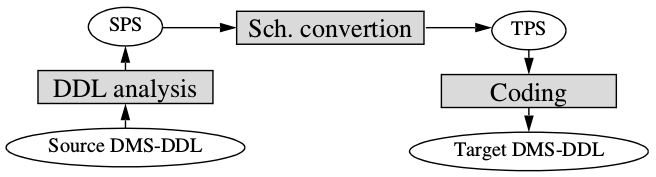
\includegraphics[width=0.9\textwidth]{../images/strategies_fig_02a.png} \\
	\tiny Quelle: \citep{henrard-2002}, Abbildung 2
\end{figure}

Durchf"uhrung auf physischer Ebene sind meist elementare Konvertierungen und m"ussen nicht zwangsweise von Analysten oder fachlich geschultem Personal vorgenommen werden. Die rein physische Konvertierung kann automatisiert durchgef"uhrt werden \citep{abiteboul-1999}.
\lb
Nachteil der physischen Konvertierung ist ein fehlender Mehrwert der entstandenen Daten \citep{henrard-2002}. Vorhandene Schemata werden soweit wie m"oglich auf andere Technologien "ubertragen. Eine fachliche und konzeptuelle Analyse der Daten bleibt aus. In diesem Fall stellt die Migration der Daten lediglich ein Umkopieren in ein neues Datenformat dar.
\lb
Die rein physische Migration eignet sich vor allem bei einem Wechsel der technischen Umgebung der Daten, etwa einem Wechsel der Version des verwendeten DMS oder einem Wechsel des Herstellers.

% ===
\subsubsection{Konzeptuell}

Anders als auf physischer Ebene werden Daten auf konzeptueller Ebene auch semantisch betrachtet. Schemata und Datenformate werden evaluiert und neu konzeptioniert. Aus der fachlichen Betrachtung der Daten ergeben sich unter Umst"anden umfangreiche "Anderungen an den Schnittstellen der Systeme. Fachliche Konvertierungen erfordern ein Umdenken. Dieses kann die fachliche Qualit"at der migrierten Daten verbessern.
\lb
Die konzeptuelle Migration der Daten f"uhrt auf vorhandenen Schemata und Datenformaten eine semantische Analyse durch. Anhand der aus dieser gewonnenen Informationen wird eine Neukonzeptionierung der Modellierung vorgenommen. Abbildung \ref{pic:conversion_conceptual} zeigt das Vorgehen w"ahrend der konzeptuellen Migration. Das Quell-DMS Schema wird mithilfe eines Database Reengineering (DBRE) analysiert \citep{henrard-2002}. Ziel dieses Vorganges ist die Bereinigung (engl.: \textit{Cleansing}) vorhandener Daten \citep{rahm-2010} \citep{hernandez-1998}. Auf Basis einer neuen Konzeptualisierung der Schemata wird die Konvertierung "ahnlich zur physischen Migration vorgenommen. Neue Formate werden in das Ziel-Format "ubertragen und kodiert. Die Konvertierung und Migration der eigentlichen Daten in die neue Umgebung erfolgt ebenfalls mithilfe von Konvertierungen. Diese ist, im Gegensatz zur physischen Konvertierung, umfangreicher. Neue Abbildungen und Modellierungen m"ussen aus vorhandenen Daten abgeleitet werden. In diesem Zusammenhang spielt auch das Reengineering der Anforderungen an die zugrundeliegenden Daten eine Rolle \citep{aiken-1994}.

\begin{figure}[h!]
	\centering
	\caption{Konzeptuelle Konvertierung}
	\label{pic:conversion_conceptual}
	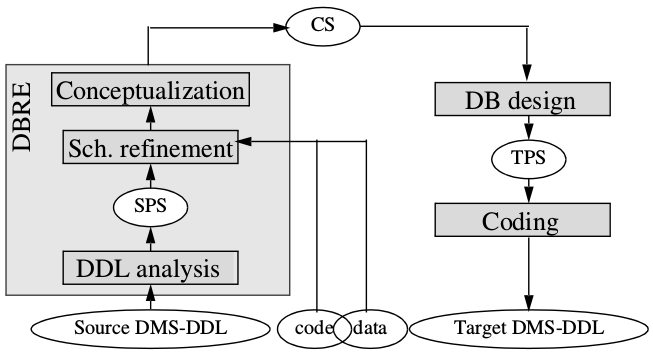
\includegraphics[width=0.9\textwidth]{../images/strategies_fig_02b.png} \\
	\tiny Quelle: \citep{henrard-2002}, Abbildung 2
\end{figure}

Auf konzeptueller Ebene spielt die fachliche Betrachtung vorhandener Daten eine wichtige Rolle. Das Verfahren ist nicht zwangsweise trivial. Analysen und konzeptuelle Konvertierung ben"otigen dabei ein gewisses Verst"andnis der Semantik entsprechender Daten.
\lb
Eine konzeptuelle Migration von Daten sorgt vor allem f"ur ein saubere Portierung vorhandener Daten. Schemata werden semantisch korrekt an neue Umgebungen und Formate angepasst. Eine potentielle S"auberung der Daten verringert unter Umst"anden Redundanzen oder nicht ben"otigte Datens"atze und -formate.
\lb
Der f"ur eine konzeptuelle Migration notwendige Aufwand ist vergleichsweise hoch. Ben"otigte Spezialisten und erforderliches fachliches Verst"andnis von Daten und Umgebung sorgen eventuell f"ur hohe Kosten.

% ==
\subsection{Anwendungsebene}

Sind Datenformate und Daten selbst konvertiert und migriert, m"ussen umgebende Softwaresysteme angepasst werden. Ver"anderte Datenformate beziehungsweise Technologien setzen oft einen ver"anderten Zugriff auf diese Daten voraus. Um den Aufwand f"ur "Anderung innerhalb der nutzenden Anwendungen m"oglichst zu reduzieren, existieren drei Strategien der Anpassung von Anwendungen. Die zeichnen sich durch unterschiedliche Ebenen der Anpassung aus. Je nach Tiefe der Anpassung liegen ihnen unterschiedliche Ans"atze zugrunde. 

% ===
\subsubsection{Wrapper}

Um den Aufwand f"ur "Anderungen innerhalb von Softwaresystemen gering zu halten, bietet sich die Implementation eines Wrappers oder Adapters an. Dieser stellt eine Schnittstelle zwischen dem urspr"unglichen, unver"anderten Anwendungssystem und der neu strukturierten Datenquelle dar. Der Wrapper wird dabei als zus"atzliche Schicht zwischen beiden Komponenten eingef"ugt. Er nimmt Aufrufe der urspr"unglichen Anwendung entgegen, "ubersetzt sie in Anfragen an die neue Datenquelle und konvertiert die Ergebnisse der Anfrage f"ur das urspr"ungliche System. Er fungiert als Vermittler zwischen beiden Systemen und erspart so den Aufwand umfangreicher "Anderungen f"ur Abfragen im Anwendungssystem.
\lb
Abbildung \ref{pic:application_wrapper} zeigt das Schema zur Nutzung eines Wrappers. Die Abstraktion erfolgt dabei auf Basis von Prozeduren zum Aufruf der neuen Datenquelle durch den Wrapper. Vor der Einbindung des Wrappers m"ussen diese in die Legacy-Anwendung eingef"ugt werden. Nur so kann der sp"atere Aufruf des Wrappers anstatt der urspr"unglichen Datenquelle erfolgen \cite{henrard-2008}. 

\begin{figure}[h!]
	\centering
	\caption{Einsatz eines Wrappers auf Anwendungsebene}
	\label{pic:application_wrapper}
	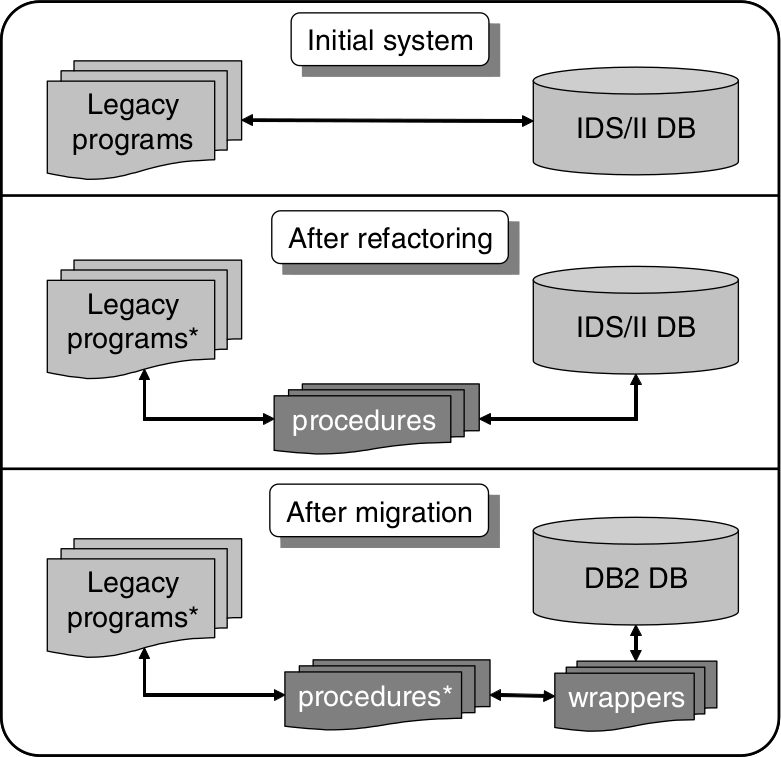
\includegraphics[width=0.5\textwidth]{../images/large_scale_fig_01.png} \\
	\tiny Quelle: \citep{henrard-2008}, Abbildung 1
\end{figure}

Ein fiktives Legacy-System dient der Illustration. Zu seinen Aufgaben geh"ort der Zugriff auf Kundendaten. Diese werden im Legacy-System mit naiven Mitteln zur Datenhaltung verwaltet \citep{henrard-2002}. Beispiel \ref{code:wrapperbefore} zeigt den urspr"unglichen Aufruf der Datenquelle. Das nachfolgende Beispiel \ref{code:wrapperafter} illustriert den neuen Zugriff auf den Wrapper. Die Anpassung an dieser Schnittstelle ist gering \citep{henrard-2002}\footnote{Die Quellcode-Beispiele auf den folgenden Seiten sind \citep{henrard-2002} entnommen und dienen lediglich der Illustration}.

\lstinputlisting[label=code:wrapperbefore,caption=Beispiel Legacy-Programm mit Aufruf der urspr"unglichen Datenquelle]{../src/wrapper_legacy.cbl}

\lstinputlisting[label=code:wrapperafter,caption=Beispiel Legacy-Programm mit Aufruf der neuen Datenquelle]{../src/wrapper_new.cbl}

Deutlicher Vorteil in der Verwendung eines Wrappers ist die notwendige geringe "Anderung des Anwendungssystems. Der Einsatz eines Wrappers gef"ahrdet die Integrit"at des nutzenden Softwaresystems nur minimal. Das Risiko wird dabei reduziert \citep{henrard-2002}. 
\lb
Durch Implementation eines Wrappers entsteht zus"atzlicher Aufwand f"ur eben diese Implementation und Integration des Wrappers in die bestehende Systemlandschaft. Die Einf"uhrung eines Wrappers ist h"aufig eine "Ubergangsl"osung. Ohne entsprechendes Verst"andnis des Anwendungssystems ist die Einf"uhrung eines Wrappers sinnvoller als tiefgreifende "Anderungen im System. 
\lb
Erfolgt der Zugriff auf eine Datenquelle an vielen Stellen im Quellcode der Legacy-Anwendung, ist die Einf"uhrung eines Wrappers mit vergleichsweise wenig Aufwand verbunden. Anders als die Anpassung von Aufrufen oder der Ver"anderung der Programmlogik, reduziert sich die Einf"uhrung eines Wrappers auf das Austauschen der Aufrufe der Datenquelle. Verarbeitung und Nutzung der Datenquelle werden vom Wrapper wie in der urspr"unglichen Quelle bereitgestellt. Die relativ simple Anpassungen beim Einsatz eines Wrappers und ein sehr geringer Aufwand f"ur die Anpassung im Legacy-System selbst sind die Vorteile bei Nutzung eines Wrappers. Entgegen dem geringen Aufwand im System selbst, erfordert die Implementation eines Wrappers entsprechendes technische Verst"andnis der neuen Datenquelle. Dies garantiert die korrekte Nutzung der Daten durch die Legacy-Anwendung. Durch den bestehenden Umfang zur Nutzung durch das Legacy-System k"onnen technische M"oglichkeiten der neuen Datenquelle unter Umst"anden nicht genutzt werden.

% ===
\subsubsection{Statements}

Eine detailliertere Anpassung der Anwendungssysteme stellt das Anpassen der Aufrufe der Datenquelle dar. Der Zugriff auf Daten erfolgt durch entsprechende Anweisungen im Quellcode einer Anwendung. Die Anpassung entsprechender Statements im Quellcode nimmt dabei die Anpassung des Anwendungssystems vor. Anpassungen in entsprechenden Statements sind der Kern dieser Strategie. Es wird lediglich der tats"achliche Zugriff auf die Datenquelle ver"andert, nicht jedoch sein Struktur. Sind umfassende "Anderungen im Bezug auf die eingesetzte Technologie durchgef"uhrt worden, reicht eine blo"se Anpassung der Statements unter Umst"anden nicht aus.
\lb
Beispiel \ref{code:statementbefore} zeigt den Aufruf der Datenquelle vor Anpassung der Statements. Die Anpassung in Beispiel \ref{code:statementeafter} verdeutlicht die Anpassung. Wo zuvor der Zugriff mit Sprachmitteln des Legacy-Systems erfolgte, sind Statements nach der Anpassung auf die Nutzung von SQL ausgelegt. Die entsprechenden Anpassungen sind umfangreicher als die Nutzung eines Wrappers \citep{henrard-2002}.

\lstinputlisting[label=code:statementbefore,caption=Aufruf der Datenquelle vor Anpassung der Statements]{../src/statementrewrite_cobol.cbl}

\lstinputlisting[label=code:statementeafter,caption=Aufruf der neuen Datenquelle: Zugriff via SQL]{../src/statementrewrite_sql.cbl}

Vorteil der Anpassung von Statements ist eine technisch saubere L"osung. Anpassungen an den Abfragen, etwa "Anderungen an SQL-Statements, sind eher simpel in der Durchf"uhrung. Die "Anderung der Statements erfordert nicht zwangsweise ein tiefgreifendes Verst"andnis des Anwendungssystems. 
\lb
Anpassungen an Statements reagieren auf eine ver"anderte Schnittstelle der Datenquelle. Gr"o"sere strukturelle oder konzeptionelle "Anderungen k"onnen jedoch nicht ber"ucksichtigt werden.
\lb
Das Anpassen von Statements im Anwendungssystem ist sinnvoll, wenn an nur wenigen Stellen im Quellcode Anpassungen vorgenommen werden. Ist etwa der Zugriff auf die Datenquelle gekapselt, ist die Anpassung nur in geringem Umfang durchzuf"uhren. Im Gegensatz zum Einsatz eines Wrappers an der Schnittstelle, ist die "Anderung von Statements eine integrierte L"osung und greift in das Anwendungssystem ein. Um die Anpassung korrekt durchf"uhren zu k"onnen, ist ein grundlegendes Verst"andnis der betreffenden Anwendung notwendig.

% ===
\subsubsection{Logik}

Um alle M"oglichkeiten neuer Datenquellen und -technologien nutzen zu k"onnen, muss unter Umst"anden die Logik des zugreifenden Anwendungssystemes ver"andert werden. Dabei werden Datenstrukturen, Algorithmen und Zugriff innerhalb der Software massiv ver"andert, um auf die neue Umgebung zu reagieren \citep{henrard-2002}.
\lb
F"ur eine Anpassung der Logik ist es erforderlich, entsprechende Passagen innerhalb der Anwendungssoftware an die neue Datenquelle anzupassen. Beispiel \ref{code:logicbefore} zeigt den urspr"unglichen Zugriff des Legacy-Systems. Die angepasste Logik ist in Beispiel \ref{code:logicafter} einzusehen. Als Unterschied zur reinen Anpassung der Statements sind die Auswirkungen auf andere Programmteile meist gr"o"ser \citep{henrard-2002}.

\lstinputlisting[label=code:logicbefore,caption=Ursp"ungliche Logik f"ur den Zugriff auf die Datenquelle]{../src/logic_before.cbl}

\lstinputlisting[label=code:logicafter,caption=Angepasste Zugriffslogik f"ur Datenquelle in SQL]{../src/logic_after.cbl}

Die Anpassung der Logik und damit potentiell die Nutzung aller M"oglichkeiten der neuen Datenquellen beziehungsweise Schnittstellen erh"oht den Nutzen der Anwendungssoftware. Kann das Softwaresystem von den neuen M"oglichkeiten Gebrauch machen, erh"oht dies m"oglicherweise den Gesch"aftswert der Komponente. 
\lb
Hinter der Anpassung der Logik eines Anwendungssystemes verbirgt sich immer ein gewisses Risiko. Je umfangreicher die "Anderungen ausfallen, desto h"oher ist das Risiko. Gerade funktionale "Anderungen, wie der Zugriff und die Arbeit mit Datenquellen, kann ein hohes Risiko beim Reengineering von Legacy-Systemen mit sich bringen.
\lb
Neben dem Einsatz eines Wrappers und der Anpassung von Statements bildet die Anpassung der Logik die umfangreichste Strategie auf Anwendungsebene. Die Umsetzung erfordert umfassendes Verst"andnis der fachlichen Logik des betreffenden Softwaresystems. Wie die bereits genannten Ans"atze stellt sich auch die Anpassung der Logik durch Vor- und Nachteile dar. Unterschiedliche Strategien und Ans"atze k"onnen die Migration auf unterschiedlichen Ebenen unterst"utzen. Welche Strategie einzusetzen ist, h"angt stark vom Kontext, dem bestehenden Legacy-System und dem technischen und fachlichen Wissen der Beteiligten eines Migrationsprojektes ab.
% !TeX spellcheck = de_DE
\section{Generelles Vorgehen}
\label{chapter:richtlinien}
%-http://www.information-management.com/specialreports/20040518/1003611-1.html
%-http://searchsmbstorage.techtarget.com/tip/Data-migration-strategies-and-best-practices
%-https://pure.fundp.ac.be/ws/files/168599/wcre02.pdf
%http://www.dtic.upf.edu/~jbisbal/publications/datasem97.pdf
%http://dc-pubs.dbs.uni-leipzig.de/files/Rahm2000DataCleaningProblemsand.pdf
%http://csis.pace.edu/~marchese/CS775/Proj1/legacyinfosys_directions.pdf
%http://www.oracle.com/technetwork/middleware/oedq/successful-data-migration-wp-1555708.pdf

%\section{Generelles Vorgehen}
%Unabh"angig von der gew"ahlten Strategie setzt die Durchf"uhrung einer Datenmigration drei grunds"atzliche T"atigkeiten voraus \citep{henrard-2002}. Diese dienen als Ger"ust der Umsetzung einer Migration. 

Die Datenmigration stellt einen risikoreichen Aufgabenbereich dar. Aus diesem Grund sollte sie nicht ohne eine vorhergehende Planungsphase und entsprechende Strukturierung durchgef"uhrt werden. Ein allgemeing"ultiges Verfahren, mit welchem das Risiko der Datenmigration reduziert werden kann, existiert jedoch nicht \citep[S.~3]{wuLawless-1997}. Dennoch existieren verschiedene Ans"atze zur Strukturierung des Migrationsprozesses. Einer dieser Ans"atze ist das von Klaus Haller, Florian Matthes und Christopher Schulz in Zusammenarbeit mit Unternehmen aus Automobil-Industrie und dem Finanzsektor entwickelte Prozessmodell f"ur Datenmigration \citep[S.~2f.]{klausMatthesSchulz-2012}. 
\lb
Dieses Prozessmodel unterteilt die Migration in vier Abschnitte: Die Initialisierung, die Migrationsentwicklung, den Testabschnitt und die Umstellung auf das neue System. F"ur jeden dieser Abschnitte werden dabei die wichtigsten T"atigkeiten dargestellt \citep[S.~5f]{klausMatthesSchulz-2012}. Je nach Unternehmen und Migrationssituation kann die tats"achliche Durchf"uhrung der T"atigkeiten variieren.
\lb
W"ahrend der Initialisierung muss die aktuelle Situation erfasst werden. Hierbei gilt es herauszufinden, um welche Art von Legacy-System es sich handelt, wo und wie Daten gespeichert sind, auf welche Art System migriert werden soll und welche Daten "ubertragen werden sollen oder m"ussen \citep[S.~7]{klausMatthesSchulz-2012}. Auf dieser Grundlage kann eine Entscheidung dar"uber getroffen werden, welche Strategien f"ur die Migration verwendet werden k"onnen. Diese Information sind somit essentiell, um das weitere Vorgehen planen zu k"onnen und eine initiale Aufwandseinsch"atzung erstellen zu k"onnen \citep[S.~7]{klausMatthesSchulz-2012}. Ebenfalls wird auf Grundlage der gesammelten Informationen eine Migrationsplattform eingerichtet. Mit Hilfe dieser Migrationsplattform werden im folgenden die ben"otigten Migrationswerkzeuge, -skripte usw. entwickelt und getestet \citep[S.~7]{klausMatthesSchulz-2012}.
\lb
Im Abschnitt zwei, der Migrationsentwicklung, wird zun"achst die vorangegange Analyse der auf dem Legacy-System vorhandenen Daten vertieft. Zu diesem Zweck wird ein Backup des Legacy-Datenbestands auf die Migrationsplatform "uberspielt. Somit kann verhindert werden, dass w"ahrend der Analyse Probleme oder St"orungen auf dem Legacy-System auftreten \citep[S.~7]{klausMatthesSchulz-2012}. Bei der Analyse ist festzustellen, welche Datenschemata und -formate auf dem Legacy-System vorhanden sind und auf dem angepassten oder neu entwickelten System vorhanden sein m"ussen. Besonders wichtig ist hierbei herauszufinden, worin sich diese Schemata voneinander unterscheiden. Dieses Wissen erm"oglicht es, Migrationsskripte zu entwickeln, mit welchen die Daten automatisiert konvertiert und "ubertragen werden k"onnen \citep[S.~7f.]{klausMatthesSchulz-2012}. 
\lb
Nachdem die Struktur der Daten analysiert worden ist, m"ussen die Daten selbst betrachtet werden. Man versucht auf diese Weise unvollst"andige, inkonsistente oder doppelte Datens"atze zu identifizieren. Um Probleme im neuen System zu vermeiden, sollten solche Datens"atze bereinigt werden. Die Bereinigung (engl.: \textit{ Cleansing}) \cite{hernandez-1998} kann entweder vor der Datenmigration auf dem Legacy-System durchgef"uhrt werden, w"ahrend der Migration mit Hilfe der Migrationsskripte oder im Anschluss auf dem bereits aktualisierten System \citep[S~7f.]{klausMatthesSchulz-2012}. Mittels dieser Bereinigung werden die inkonsisten und unvollst"andigen Datens"atze repariert und redundante Datens"atze entfernt \citep[S.~7f.]{rahm-2010}. 
\lb
Die w"ahrend der Migrationsentwicklung entwickelten Skripte m"ussen anschlie"send im Testabschnitt ausgiebig auf ihre Funktionalit"at "uberpr"uft werden. Entsprechende Tests werden auch hier auf der Migrationsplattform ausgef"uhrt \citep[S.~8f.]{klausMatthesSchulz-2012}. Gefundene Fehler werden korrigiert, woraufhin die Migrationsskripte erneut "uberpr"uft werden m"ussen. Dieser Prozess wird solange wiederholt, bis die Migrationsskripte fehlerfrei sind und deren Ergebnisse als korrekt validiert wurden \citep[S.~8f.]{klausMatthesSchulz-2012}.
\lb
Abschlie"send folgt die Umstellung auf das neue System. Dieser Abschnitt beinhaltet die Migration vom Legacy- auf das neue System mit Hilfe der zuvor entwickelten Migrationsskripte. Je nach gew"ahlter Vorgehensweise bleibt das Legacy-System bis zum Abschluss der Migration und Sicherstellung der Funktionalit"at des zuk"unftigen Systems im Einsatz \citep[S.~107]{bisbal-1999}. 
\lb
Nachdem die Datenmigration abgeschlossen wurde, ist es in der Regel sinnvoll, einen Erfahrungsbericht zu erstellen. In diesem soll festhalten werden, in welchen Phasen der Migration es zu Problemen kam und wie diese behoben wurden. Auf diese Weise soll der Migrationsprozess im Unternehmen aktiv verbessert werden. Ebenfalls soll sichergestellt werden, dass in zuk"unftigen Migrationsprojekten nicht dieselben Probleme auftreten \citep[S.~10]{klausMatthesSchulz-2012}.



% !TeX spellcheck = de_DE
\section{Einf"uhrungsstrategien der Datenmigration}
\label{chapter:vorgehensweisen}
%TODO Julian
%http://www.information-management.com/specialreports/20040525/1003961-1.html
%http://edepositireland.ie/bitstream/handle/2262/27040/The%20Butterfly%20Methodology%20a%20gateway-free%20approach%20for%20migrating%20legacy%20information%20systems.pdf?sequence=1&isAllowed=y
%http://www.dtic.upf.edu/~jbisbal/publications/icsc97.pdf
%https://pure.fundp.ac.be/ws/files/168599/wcre02.pdf
%http://www.dtic.upf.edu/~jbisbal/publications/datasem97.pdf
%http://csis.pace.edu/~marchese/CS775/Proj1/legacyinfosys_directions.pdf

%Quellen hinzuf"ugen
% neue System -> Zielsystem + Definition?

Das vom Unternehmen angewandte Prozessmodell beinhaltet ebenso die Wahl einer Einf"uhrungsstrategie, welche den technischen Ablauf und die Einf"uhrung der Datenmigration beschreibt. Da die gew"ahlte Einf"uhrungsstrategie den weiteren Verlauf des Prozessmodells beeinflusst, wird diese in einer fr"uhen Phase, nachdem die Kerndaten von Legacy- und neuem System analysiert wurden, ausgew"ahlt. Eine sp"atere Revision dieser Entscheidung ist nicht oder nur sehr schwer m"oglich. Allerdings kann nicht jede Einf"uhrungsstrategie in jedem Kontext f"ur die Durchf"uhrung einer Datenmigration genutzt werden. Im Folgenden werden zu diesem Zweck drei Einf"uhrungsstrategien mit ihren jeweiligen Vor- und Nachteilen vorgestellt. 

\subsection{Big-Bang-Ansatz}

Der \textit{Big-Bang} oder auch als \textit{Cold Turkey} bekannte Ansatz ist wohl das "alteste Model zur Durchf"uhrung einer Datenmigration. Nachdem das Legacy- und das neue System ausreichend analysiert und deren Unterschiede gefunden wurden, wird beim Big-Bang-Ansatz das Legacy-System abgeschaltet. Somit m"ussen auch s"amtliche vom Legacy-System gest"utzte Gesch"aftsprozesse unterbrochen werden \citep[S.~4]{wuLawless-1997}. 
\lb
W"ahrend dieser Unterbrechung wird ein Dump des gesamten Datenbestands des Legacy-Systems angelegt\footnote{Ein \textit{Dump} (Auszug) ist ein Abbild des Speicherzustandes etwa einer Datenbank zu einem bestimmten Zeitpunkt}. Dieser wird anschlie"send mittels der hierf"ur entwickelten Migrationsskripte in das neue System "ubertragen \citep[S.~3]{brodie-1993}. Bis die Datenmigration abgeschlossen ist, kann weder das neue noch das Legacy-System im Unternehmen eingesetzt werden. Daraus resultiert ein Zeitraum, in welchem das Unternehmen ohne ein lauff"ahiges System auskommen muss und somit stark in seiner Gesch"aftsf"ahigkeit eingeschr"ankt ist \citep[S.~3f.]{brodie-1993}.
\lb
Die Vorteile diese Ansatzes beschr"anken sich auf das verbesserte Programmverst"andnis, die Performance und die bessere Wartbarkeit des neuen Systems, nachteilig hingegen ist ein hohes Risiko bei Fehlschlag der Einf"uhrung \citep[S.~105]{bisbal-1999}. Das hohe Risiko des Big-Bang-Ansatz besteht vor allem darin, dass der gesamte Datenbestand auf einmal migriert wird. Eventuell auftretende Fehler k"onnen somit erst Festgestellt werden wenn die Datenmigration abgeschlossen ist, wodurch der ganze Prozess wiederholt werden muss. Neben dem hohen Risiko besteht bei Nutzung Big-Bang-Ansatzes allerdings auch noch der Nachteil der zeitweisen Unterbrechung aller vom Legacy- bzw. dem neuen System unterst"utzten Gesch"aftsprozesse um die Datenmigration durchf"uhren zu k"onnen \citep[S.~4]{wuLawless-1997}.
\lb
Zusammenfassend bietet der Big-Bang-Ansatz auf der einen Seite eine unkomplizierte Datenmigration. Auf der anderen Seite jedoch stehen ein hohes Risiko bei der Einf"uhrung sowie Ausfallzeiten w"ahrend der Einf"uhrung der "Anderungen. In diesem Zeitraum k"onnen Gesch"aftst"atigkeiten nur eingeschr"ankt oder gar nicht durchgef"uhrt werden. Der Big-Bang-Ansatz findet aufgrund des hohen Risikos in der heutigen Zeit sehr selten Anwendung in Unternehmen.

\subsection{Chicken-Little-Ansatz}

Der Chicken-Little-Ansatz stellt eine weitere Einf"uhrungsstrategie zur Datenmigration dar. Entwickelt wurde dieser Ansatz von Michaell Brodie und Michael Stonebraker im Rahmen des 1991 begonnenen DARWIN-Projekts der University of California in Berkeley \citep{zoulafy-2002}. Der Chicken-Little-Ansatz ist im Gegensatz zum Big-Bang-Ansatz ein inkrementelles Vorgehen zur Datenmigration. Durch das inkrementelle Vorgehen sollen Schw"achen des Big-Bang-Ansatzes beseitigt werden. So k"onnen bei Chicken-Little-Ansatz beispielsweise Ausfallzeiten der von Legacy- bzw. neuen System unterst"utzten Gesch"aftsprozesse w"ahrend der Datenmigration vermieden oder zumindest auf ein minimum reduziert werden \citep{zoulafy-2002}.
\lb
Das inkrementelle Vorgehen erm"oglicht hierbei eine Entwicklung und Einf"uhrung aller "Anderungen im Rahmen kleinerer Module. Entwickelt und eingef"uhrt werden zun"achst wenige Anpassungen. Inkrementell k"onnen weitere Funktionalit"aten des Legacy-Systems und damit der migrierten Daten "ubertragen werden \citep[S.~2]{wuLawless-1997}.
\lb
Um auch w"ahrend der Datenmigration die kontinuierliche Arbeit mit Softwaresystemen zu erm"oglichen, kommt beim Chicken-Little-Ansatz ein sogenanntes Gateway zum Einsatz. Dieses Gateway verbindet Legacy- und das neue System nach "Anderung oder Neuentwicklung miteinander und koordiniert deren Kommunikation untereinander. Somit k"onnen das neue und das Legacy-System solange parallel ausgef"uhrt werden, bis das neue System alle Daten enth"alt und alle Funktionalit"aten "ubernehmen kann \citep[S.~2]{wuLawless-1997}. Die neuen Daten, die w"ahrend der Zeit entstehen in der das neue System noch nicht alle Funktionen "ubernommen hat, werden dabei auf dem f"ur diese Funktion zust"andigen System gespeichert. Folglich werden Daten, welche durch bereits ans neue System "ubertragene Funktionen erstellt worden sind auch dort gespeichert und nicht mehr auf dem Legacy-System \citep[S.~2]{wuLawless-1997}. In gewissen Kontexten ist es sinnvoll, Daten zeitweise in beiden Systemen zu pflegen. Urspr"ungliche Schemata und Datenquellen werden erst verworfen, sobald zuk"unftige System diese Aufgaben verl"asslich erf"ullen k"onnen.
\lb
Das Gateway erf"ullt nun zwei Aufgaben beim "Ubertragen der Daten an das neue System. Zum einen ist dies das Bereitstellen der noch nicht migrierten Daten an das neue System und zum Anderen das Bereitstellen der bereits migrierten Daten an das Legacy-System. Ersteres wird auch als umgekehrtes Gateway (engl.: \textit{reverse Gateway}) und letzteres als Vorw"arts-Gateway (engl.: \textit{forward Gateway}) bezeichnet \citep[S.~2]{wuLawless-1997}. Je nachdem, wie stark sich Datenbankschemata von Legacy- und neuem System unterscheiden, stellen vorw"arts- und umgekehrtes Gateway unterschiedlich komplexe Module dar. Mit steigender Komplexit"at dieser Module sinkt allerdings auch die Performanz der Systeme w"ahrend der Migrationsphase \citep[S.~109]{bisbal-1999}.
\lb
"Ahnlich dem Big-Bang-Ansatz, bietet der Chicken-Little-Ansatz die erwarteten Verbesserungen in Performance, Wartbarkeit sowie im Verst"andnis des Systems \citep[S.~108]{bisbal-1999}. Allerdings fallen bei Einsatz des Chicken-Little-Ansatzes keine Ausfallzeiten, in denen weder mit Legacy- noch mit dem neuen System gearbeitet werden kann, an. Erm"oglicht wird dies durch den Einsatz des Gateways, wodurch auch w"ahrend der Migrationsphase mit dem gesamten System gearbeitet werden kann \citep[S.~2]{wuLawless-1997}. Dar"uber hinaus bietet der Chicken-Little-Ansatz noch weitere Vorteile. Es muss beispielsweise nicht das gesamte Legacy-System auf einmal ersetzt werden. Stattdessen kann dieses Modul f"ur Modul erneuert werden. Dies erleichtert Entwicklung bzw. Anpassung des neuen Systems \citep[S.~3]{brodie-1993}. Die inkrementelle Anpassung des neuen Systems bietet auch Vorteile in der Fehlerbehandlung. So m"ussen bei Auftreten von Fehlern nur die entsprechenden Schritte wiederholt werden. Wenn etwa ein Problem bei der Datenmigration eines entwickelten Moduls auftritt, muss nach der Fehlerbehebung lediglich die Datenmigration von diesem Modul wiederholt werden. Durch die Fehlerbehebung gewonnene Kenntnisse k"onnen ebenfalls in den n"achsten Schritten genutzt werden, um Probleme zu vermeiden, bevor diese entstehen \citep[S.~3]{brodie-1993}.
\lb
% je nach LIS unterschiedlich schwer durchzuf"uhren
Neben den genannten Vorteilen hat der Chicken-Little-Ansatz auch einige Nachteile aufzuweisen. Zwar erlaubt es der Einsatz eines Gateways w"ahrend der Migrationsphase, mit einem kombinierten System zu arbeiten, daf"ur stellt die Entwicklung des Gateway eine Herausforderung dar. Sie zieht unter Umst"anden hohe Kosten mit sich und erfordert eine hohes fachliches Verst"andnis beider Systeme. Daten, welche auf beiden Systemen vorhanden sind, m"ussen konsistent gehalten werden. Um die Interoperabilit"at der beiden Systeme zu erm"oglichen, muss das Gateway semantische und technische Verkn"upfungen beider Schemata herstellen. Je unterschiedlicher die Datenbankschemata von Legacy- und neuem System sind, desto komplexer erscheint diese Aufgabe \citep[S.~2f.]{wuLawless-1997}. Dar"uber hinaus muss bei komplexeren Gateways auch mit Einbu"sen im Hinblick auf Performance gerechnet werden, wenn ein vorw"arts- beziehungsweise umgekehrtes Gateway zum Einsatz kommt \citep[S.~109]{bisbal-1999}.
\lb
Alles in Allem betrachtet bietet der Chicken-Little-Ansatz viele Vorteile. Die inkrementelle Herangehensweise minimiert viele Risiken und Probleme, wie z.B. die Ausfallzeiten des Big-Bang-Ansatzes. Aus diesem Grund eignet sich Chicken-Little auch zum Einsatz in gr"o"seren Unternehmen. Dennoch muss bedacht werden, dass die Durchf"uhrung des Chicken-Little-Ansatzes auch schnell sehr komplex werden kann.

\subsection{Butterfly-Ansatz}


% versucht Problematik des Gateway zu umgehen
% Daten des Legacy-System werden in TempStorages "ubertragen
% Legacy-System bleibt bis Abschluss im Betrieb
% Nach "ubertragung der initialen Daten mittels temp0, wird temp1 mit den neuen Daten angelegt ...
% temp werden mit der Zeit immer kleiner bis temp so klein ist das dieses ausreichend schnell "ubertragen werden kann -> Abschalten des Legacy-System und abschließende "ubertragung
% minimal Downtime f"ur finale Daten"ubertragung bis das neue System eingesetzt werden kann

Im Rahmen des MILESTONE-Projekt, welches 1996 startete, wurde in einer Kooperation vom Trinity College Dublin, Broadcom \'{E}ireann Research, Telecom \'{E}ireann und Ericson der sogenannte Butterfly-Ansatz entwickelt \citep[S.~202]{wuLawlessBisbal-1997}. Der Butterfly-Ansatz ben"otigt keine Gateways, die zwischen den Systemen vermitteln \citep[S.~202]{wuLawlessBisbal-1997}. Folglich ist es auch nicht m"oglich, dass w"ahrend der Datenmigration auf beiden Systemen gearbeitet werden kann. Allerdings ist diese Aussage nicht mit einer l"angeren Ausfallzeit, wie beim Big-Bang-Ansatz, gleichzusetzen. Stattdessen wird beim Butterfly-Ansatz mit tempor"aren Datenspeichern gearbeitet, die die kontinuierliche Arbeit mit dem Legacy-System w"ahrend der Datenmigration erm"oglichen. Das neue System kommt erst zum Einsatz. sobald alle Daten auf dieses "ubertragen worden sind, bis dies geschehen ist, bleibt das Legacy-System im Einsatz \citep[S.~3]{wuLawless-1997}.
\lb
Zu Beginn der Datenmigration wird beim Butterfly-Ansatz der aktuelle Datenbestand des Legacy-Systems eingefroren. Ab diesem Zeitpunkt k"onnen auf dem Legacy Datenbestand nur noch Lese-Aktionen durchgef"uhrt werden, jedoch k"onnen dort keine neuen Daten mehr hinterlegt werden \citep[S.~202]{wuLawlessBisbal-1997}. Um dennoch mit dem Legacy-System weiterarbeiten zu k"onnen, bedient sich der Butterfly-Ansatz eines tempor"aren Speichers sowie eines \textit{Data-Access-Allocator} (DAA). Dieser Data-Access-Allocator enth"alt Informationen dar"uber, wo welche Daten im eingefrorenen Datenbestand zu finden sind und welcher tempor"arer Speicher gerade aktiv ist \citep[S.~202]{wuLawlessBisbal-1997}. Wie in Abbildung \ref{pic:datemigration_Butterfly} zeigt, wird der Data-Access-Allocator zwischen die Anwendungen und Dienste des Legacy-System und deren Datenbank geschaltet. Werden nun neue Daten ins Legacy-System eingegeben oder werden vorhandene bearbeitet, sorgt der Data-Access-Allocator daf"ur, dass das die entsprechenden Daten aus dem eingefrorenen Datenbestand gelesen werden und neue oder im aktuellen tempor"aren Speicher abgelegt werden \citep[S.~202]{wuLawlessBisbal-1997}.
\lb

\begin{figure}
	\centering
	\caption{Datenmigration mittels des Butterfly-Ansatzes}
	\label{pic:datemigration_Butterfly}
	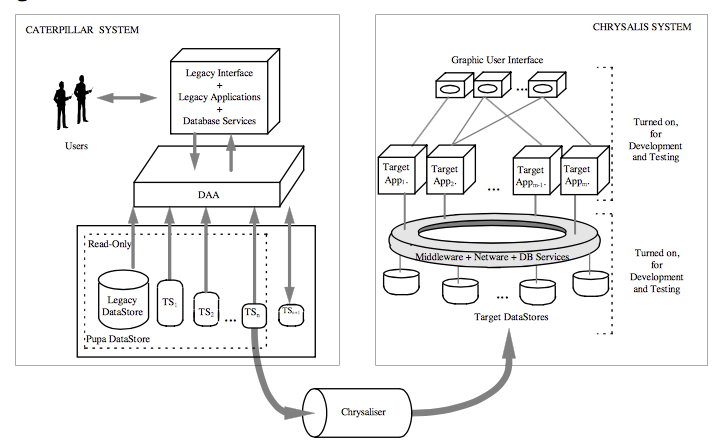
\includegraphics[width=1.0\textwidth]{../images/vorgehensweisen_fig_01.png} \\
	\tiny Quelle: \citep[S.~6]{wuLawless-1997}, Abbildung 11
\end{figure}

Durch Data-Access-Allocator und tempor"are Speicher wird sichergestellt, dass w"ahrend der Datenmigration mit dem Legacy-System normal weitergearbeitet werden kann. F"ur die "Ubertragung der Daten auf das neue System wird allerdings noch ein \textit{Daten-"-Transformator}, ein sogenannter \textit{Chrysaliser} ben"otigt \citep[S.~202]{wuLawlessBisbal-1997}. Dieser Chrysaliser "ubernimmt die Rolle der Migrationsskripte. Er enth"alt die Informationen "uber die Datenbankschemata des Legacy- und des neuen Systems sowie die Schemata des Legacy-System, welche umgewandelt werden m"ussen \citep[S.~202]{wuLawlessBisbal-1997}. 
\lb
Mit Hilfe des Chrysaliser werden nun die Daten aus dem eingefrorenen Datenbestand an das neue System "ubertragen. Sobald alle Daten aus dem eingefrorenen Datenbestand "ubertragen wurden, wird ein weiterer tempor"arer Speicher \texttt{t2} angelegt und der Datenbestand des alte tempor"are Speicher eingefroren. Anschlie"send muss der Data-Access-Allocator entsprechend angepasst werden \citep[S.~202]{wuLawlessBisbal-1997}. Der Chrysaliser kann nun damit beginnen, den tempor"aren Speicher \texttt{t1} auf das neue System zu "ubertragen. Ist auch \texttt{t1} "ubertragen wird \texttt{t2} eingefroren und ein tempor"arer Speicher \texttt{t3} f"ur neue im Legacy-System angelegte Daten angelegt (siehe Abbildung \ref{pic:datemigration_Butterfly}) \citep[S.~202]{wuLawlessBisbal-1997}. Mit jeder neuen Iteration des tempor"aren Speichers reduziert sich dessen Gr"o"se. Dieser Umstand l"asst sich darauf zur"uckf"uhren, dass in der Zeit die f"ur die Migration des initialen Datenbestands ben"otigt wird, der Datenbestand in der Regel nicht verdoppelt. Der tempor"are Speicher \texttt{t1} m"usste somit auch kleiner sein als der initiale Datenbestand des Legacy-Systems. Analoges gilt f"ur die folgenden Iterationen des tempor"aren Speichers: \textbf{$t_n <t_{n+1}$} \citep[S.~202]{wuLawlessBisbal-1997}. 
\lb
Dieser Vorgang wird solange wiederholt, bis der tempor"are Speicher eine zu Beginn der Datenmigration festgelegte Gr"o"se erreicht. Wenn der tempor"are Speicher diese Gr"o"se nun erreicht und es an der Zeit ist, diesen durch den Chrysaliser auf das neue System zu migrieren, wird dieser wie auch schon seine Vorg"anger eingefroren. Allerdings wird kein neuer tempor"arer Speicher eingerichtet. Stattdessen wird ab diesem Zeitpunkt der Betrieb auf dem Legacy-System eingestellt damit die letzten Daten migriert werden k"onnen \citep[S.~202]{wuLawlessBisbal-1997}. Aus diesem Grund sollte die Gr"o"se des letzten tempor"aren Speichers so gew"ahlt werden, dass eine schnelle Migration von diesem aus m"oglich ist. Auf diese Weise kann die Ausfallzeit des Systems minimal gehalten werden \citep[S.~202]{wuLawlessBisbal-1997}. Nachdem die Datenmigration abgeschlossen ist, kann das neue System in Betrieb genommen und das Legacy-System endg"ultig abgeschaltet werden \citep[S.~204]{wuLawlessBisbal-1997}.
\lb
Neben den allgemeinen Vorteilen, wie z.B. verbesserter Wartbarkeit, bietet der Butterfly-Ansatz eine minimale Beeintr"achtigung durch Systemausf"alle, in denen die vom System unterst"utzten Gesch"aftsprozesse nicht ausgef"uhrt werden k"onnen. Durch die Wahl einer entsprechend kleinen Gr"o"se des letzten tempor"aren Speichers kann die anfallende Ausfallzeit flexibel an die Bed"urfnisse des Unternehmens angepasst werden \citep[S.~204f.]{wuLawlessBisbal-1997}. Dar"uber hinaus kann beim Butterfly-Ansatz im Gegensatz zu anderen Ans"atzen die f"ur die Migration ben"otigte Gesamtzeit relativ sicher anhand des initialen Datenbestands des Legacy-Systems sowie der Geschwindigkeit von Data-Access-Allocator und Chrysaliser eingesch"atzt werden. Durch die Einsch"atzung des Zeitaufwands ist es dem Unternehmen m"oglich, die Migration besser zu planen und so unn"otige Problematiken zu vermeiden. Beispielsweise kann verhindert werden, dass die Migration des System in eine Zeit f"allt, in welcher das System st"arker als normal beansprucht wird \cite[S.~204]{wuLawlessBisbal-1997}. Des Weiteren entf"allt beim Butterfly-Ansatz die Notwendigkeit zur Entwicklung eines Gateways, um w"ahrend der Datenmigration weiterarbeiten zu k"onnen, da das Legacy-System bis zum Abschluss im Betrieb bleibt. Dies bietet ebenfalls den Vorteil, dass keine Probleme mit der Konsistenz von Daten auftreten k"onnen \citep[S.~3]{wuLawless-1997}.
\lb
Allerdings hat der Butterfly-Ansatz auch Nachteile, welche bei der Entscheidung, welche Einf"uhrungsstrategie verwendet werden soll, ber"ucksichtigt werden m"ussen. So muss zwar kein komplexes Gateway entwickelt werden, an dessen Stelle allerdings ein Data-Access-Allocator, welcher tempor"are Speicher einrichtet und die Anfragen aus dem Legacy-System entsprechend umleiten kann. Ebenso ein Chrysaliser, welcher die Daten auf das neue System "ubertragen kann \citep[S.~3]{wuLawless-1997}. Sowohl Data-Access-Allocator als auch Chrysaliser sind entscheidend daf"ur, wie schnell und sicher eine Migration mit dem Butterfly-Ansatz durchgef"uhrt werden kann. Aus diesem Grund wird auch hier ein hohes technisches Verst"andnis f"ur die Entwicklung ben"otigt \citep[S.~204]{wuLawlessBisbal-1997}. Des Weiteren kann es passieren, dass je nach zu migrierenden Legacy-System ein gro"se Anzahl an tempor"aren Speichern ben"otigt wird. Folglich kann es zu einem hohen Hardwarebedarf f"ur Speicher kommen, wodurch wiederum die Kosten der Migration in die H"ohe getrieben werden \citep[S.~109f.]{bisbal-1999}.
\lb
Zusammenfassend betrachtet stellt der Butterfly-Ansatz wie auch schon Big-Bang und Chicken-Little keine allgemeing"ultige L"osung dar. Auch hier muss beachtet werden, dass der Butterfly-Ansatz sich nicht zur Migration mit jedem Legacy-System eignet. 

% !TeX spellcheck = de_DE
\section{Fazit}
\label{chapter:fazit}

Die Datenmigration im Kontext des Reengineering ist kein triviales Verfahren. Durch die Vielschichtigkeit von Unternehmen und Softwaresystemen eignen sich in unterschiedlichen Kontexten verschiedene Strategien. Als h"aufig untersch"atztes Verfahren hat die Migration von Daten einen hohen Gesch"aftswert, etwa die Erhaltung gesch"aftskritischer Kundendaten. Mangelnde Planung und undefinierte Herangehensweisen k"onnen Projekte der Datenmigration scheitern lassen. Durch das Nutzen von Strategien zur Durchf"uhrung, Planungsrichtlinien und Einf"uhrungsstrategien kann die Migration strukturiert werden.
\lb
Sowhol die Migration der Daten selbst, als auch die Anpassung umliegender Anwendungen und Softwaresysteme spielt eine zentrale Rolle. Unterschiedliche Konzepte bieten jeweils fundierte Strategien f"ur die Migration. Aspekte wie fachliches und technisches Wissen um Schnittstellen und Datenmodelle k"onnen Grundlage f"ur die Auswahl einer Strategie sein. Der zuk"unftige Gesch"aftswert nach durchgef"uhrten "Anderungen kann bei der Auswahl ebenfalls eine Rolle spielen. So k"onnen neue technische M"oglichkeiten nach Austausch der Datenbank-Plattform effizientere Schnittstellen bereitstellen und Zugriffe redundanzfrei gestalten.
\lb
Bei der Durchführung und bei der Wahl ist stets zu beachten, dass es keine universelle Lösung gibt, die immer das beste Ergebnis liefert. Vielmehr muss für jedes Unternehmen jede mögliche Vorgehensweise genau betrachtet werden. So bietet sich beispielsweise der Chicken-Little-Ansatz für ein Unternehmen an, das vorhat sein Legacy-System Anwendung für Anwendung nacheinander zu ersetzen. Wenn das Unternehmen allerdings die komplett auf ein neues System wechseln will, dabei aber die Ausfallzeiten minimal halten will eignet sich vielleicht der Butterfly-Ansatz doch besser. 
\lb
Um die richtige Entscheidung treffen zu können muss immer die gesamte Situation analysiert werden. Was für ein Unternehmen liegt vor, sollen nur die Daten auf ein neues System migriert werden oder muss das neue System auch erst noch entwickelt werden? Für diese Fragen und weitere müssen Antworten gefunden werden. Aus diesem Grund stellt ein geplantes Vorgehen eine wichtige Rolle für die erfolgreiche Datenmigration. Aber auch hierbei ist anzumerken, dass es auch hier keine allgemein gültiges Planung existiert und diese an die Gegebenheiten angepasst werden muss. 
\lb
Die Durchf"uhrung der Datenmigration ist ein dynamisches Verfahren. Im speziellen Kontext von Unternehmen, Projektteam und vorhandenen Systemen sind zu nutzenden Strategien individuell abzustimmen. Gerade die Ungewissheit, welche Legacy-System h"aufig mit sich bringen, erm"oglichen keine statische Auswahl einer Musterl"osung f"ur die Datenmigration.


% ===========================================================================================================
% ======= END CONTENT =======================================================================================
% ===========================================================================================================

% === BIB ===
\newpage
%\bibliographystyle{alphadin}
\bibliographystyle{dinat}
\addcontentsline{toc}{section}{\bibname}

\bibliography{../bib/mproj}
\end{document}